\chapter{Iteración 5: Diseño final de hardware} % (fold)
\label{cha:iteracion_5}

\section{Introducción} % (fold)
\label{sec:introduccion}

Los distintos inconvenientes que surgieron en el desarrollo de las iteraciones 2, 3 y 4, nos obligo a analizar distintas alternativas para lograr cumplir por completo con los requerimientos 1.1 y 1.3. En iteraciones pasadas, se configuro el software y el hardware de la plataforma para poder tomar señales de hasta 2 contadores y hasta 4 señales en modo diferencial de 4 respectivos sensores. Esto no cumple con el numero minimo de 4 contadores y 8 canales diferenciales. Si se duplicaran los recursos, llegariamos a la cantidad requerida.

En esta iteración, intentamos aumentar las prestaciones de la plataforma duplicando los recursos de la placa construida en la iteración 3. Duplicando los recursos, alcanzariamos los requerimientos de cantidad de contadores y canales de medición diferenciales.

% section introduccion (end)

\section{Requerimientos de la iteración} % (fold)
\label{sec:requerimientos_de_la_iteracion}

A continuacion, listamos los requerimientos de esta iteracion.

\begin{itemize}
  \item Se deberían poder convertir a digital en modo canal unico o diferencial, datos analógicos provenientes de hasta 8 sensores. [1.1]
  \item Se deberían poder contar eventos de hasta 4 señales externas. [1.3]
\end{itemize}

% section requerimientos_de_la_iteracion (end)

\section{Desarrollo} % (fold)
\label{sec:desarrollo}

\subsection{Diseño Esquemático}
\label{sub: diseño_esquematico2}

Para simplificar la explicación del diagrama, lo que haremos en esta sección es dividir el circuito entero en subcircuitos mas simples.

\subsubsection{Entradas Analógicas}
\label{subsub: entradas_analogicas2}

Las entradas analógicas con sus filtros se mantuvieron exactamente igual que en el diseño de la primera placa. Para cada una de las entradas se le colocaría un filtro pasa-bajo RC como se muestra en la figura \ref{fig:esquematicoFiltro}.

Mostramos en la figura \ref{fig:esquematicoFiltro2} como quedan todas las entradas analógicas de un solo chip (en el otro es exactamente igual), podemos ver 8 entradas analógicas, cada una con su respectivo filtro. Además podemos observar 2 pines llamados PINHD\_AGND\_2, son dos accesos a la masa digital para aquellos sensores que necesiten estar referenciado a masa (colocamos dos masa analógicas para cada uno de los chips).

Del lado derecho del microcontrolador hay dos entradas denominadas VREF+ y VREF-, que nos sirven para manejar los niveles de tensión de referencia para la conversión que usara el ADC.

\begin{figure}[H]
\centering
  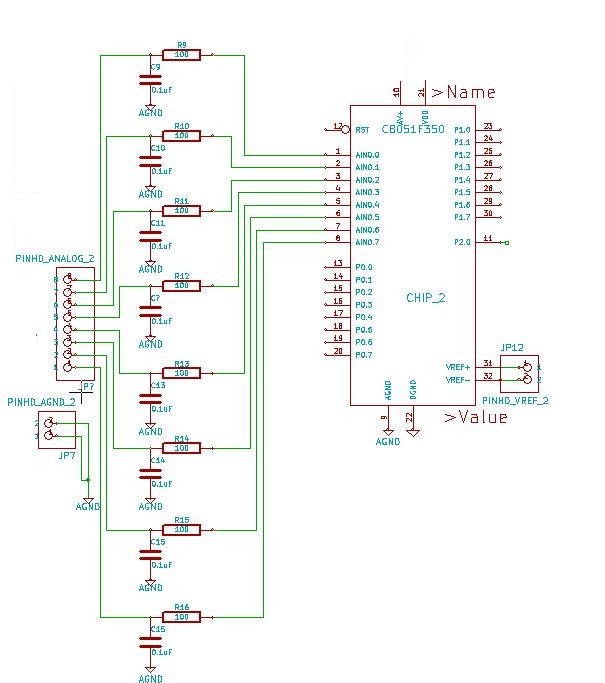
\includegraphics[width=1.10\textwidth, height = 9cm]{esquematicoFiltro2}
  \caption{Esquemático del Circuito Completo de entradas analogicas.}\label{fig:esquematicoFiltro2}
\end{figure}

% subsubsection entradas_analogicas2 (end)

\subsubsection{Circuito de entradas Digitales}
\label{subsub:entradas_digitales}

Como podemos ver en la figura \ref{fig:esquematicoDigital2} colocamos 16 entradas/salidas digitales para el microcontrolador. Cada chip tiene las mismas 16 entradas.

\begin{figure}  [H]
\centering
  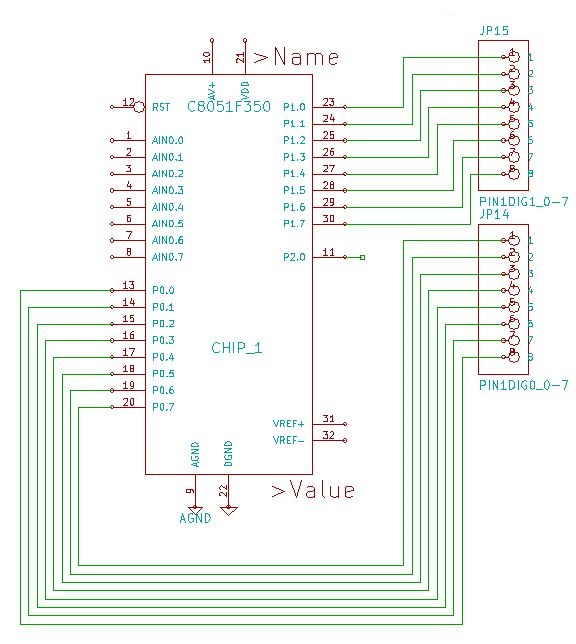
\includegraphics[width=1.0\textwidth, height = 10cm]{esquematicoDigital2}
  \caption{Esquemático del Circuito Completo de entradas/salidas digitales.}\label{fig:esquematicoDigital2}
\end{figure}


% subsubsection entradas_digitales (end)

\subsubsection{Circuito Salida Serial}
\label{subsub:salida_serial2}

La idea de tener una placa a la que se conecten varios sensores analógicos y digitales es que se pueda colocar el lugares remotos, por lo que decidimos que la salida serial deje de ser RS-232 y colocarle dos salidas seriales nivel TTL con un RX y un TX para cada microcontrolador, además colocando éste tipo de salida se ahorra mucho espacio, así pudimos reducir el tamaño de la placa. Las salidas seriales se encuentran conectadas directamente en los pines de salidas dijitales P0.4 (Tx) y P0.5(Rx).

% subsubsection salida_serial2 (end)

\subsubsection{Circuito para Debugger y Programación} % (fold)
\label{subsub:debugger_programacion2}

Para programar cada uno de los microcontroladores en principio se pensó en colocar dos entradas para el debugger de SiliconLabs, pero nos consumía mucho espacio y el cambio para programar uno y otro se hubiera hecho molesto. Por lo que decidimos poner uno solo, y utilizarlo para los dos microcontroladores, con un jumper de tres pines, para tener la opción de elegir que micro programar.
En la figura \ref{fig:esquematicoDebugger2} vemos en uno de los C8051f352 como queda conectado el modulo de debugger/programación.

\begin{figure}  [H]
\centering
  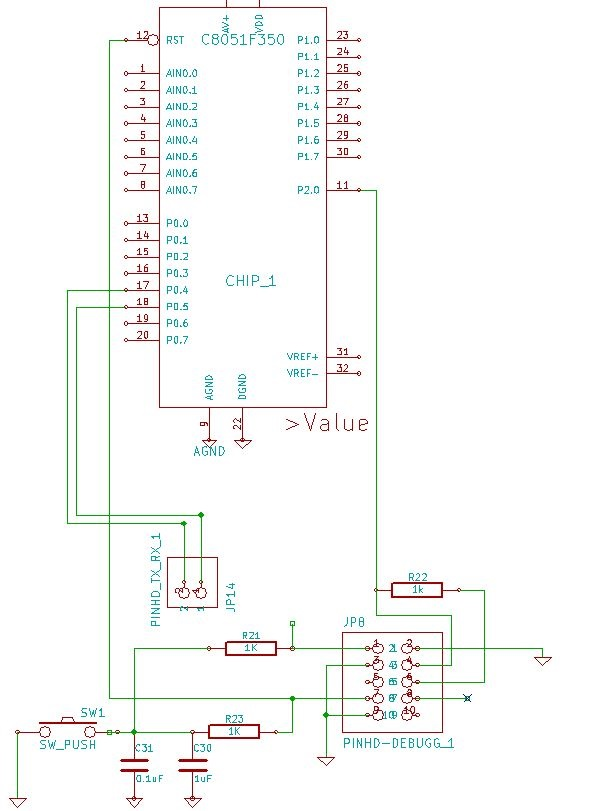
\includegraphics[width=1.0\textwidth, height = 8cm]{esquematicoDebugger2}
  \caption{Esquemático del Circuito para la programación de los microcontroladores de la placa.}\label{fig:esquematicoDebugger2}
\end{figure}


% subssubection debugger_programacion2 (end)

\subsubsection{Circuito de Potencia}
\label{subsub: circuito_potencia2}

Para el circuito de potencia hicimos lo mismo que con el debugger: colocamos una sola entrada y un solo regulador para toda la placa y asi, alimentamos los dos microcontroladores. También colocamos un jumpers (JMP3), se utiliza para decidir si alimentamos la placa con una fuente externa o con el debugger/programador de SiliconLabs. 
Sabemos que el principal problema de un sistema embebido es su consumo de energía, por lo que colocamos dos jumpers más, uno para cada una de las entradas de alimentación del segundo microcontrolador (JP4 AV+ y JP5 para VDD). Entonces así podemos elegir desconectar un chip y ahorrar el consumo de energía que este provocaría. 

En la figura \ref{fig:esquematicoPotencia2} se muestra como queda el esquemático del circuito de potencia.

\begin{figure}[H] 
\centering
  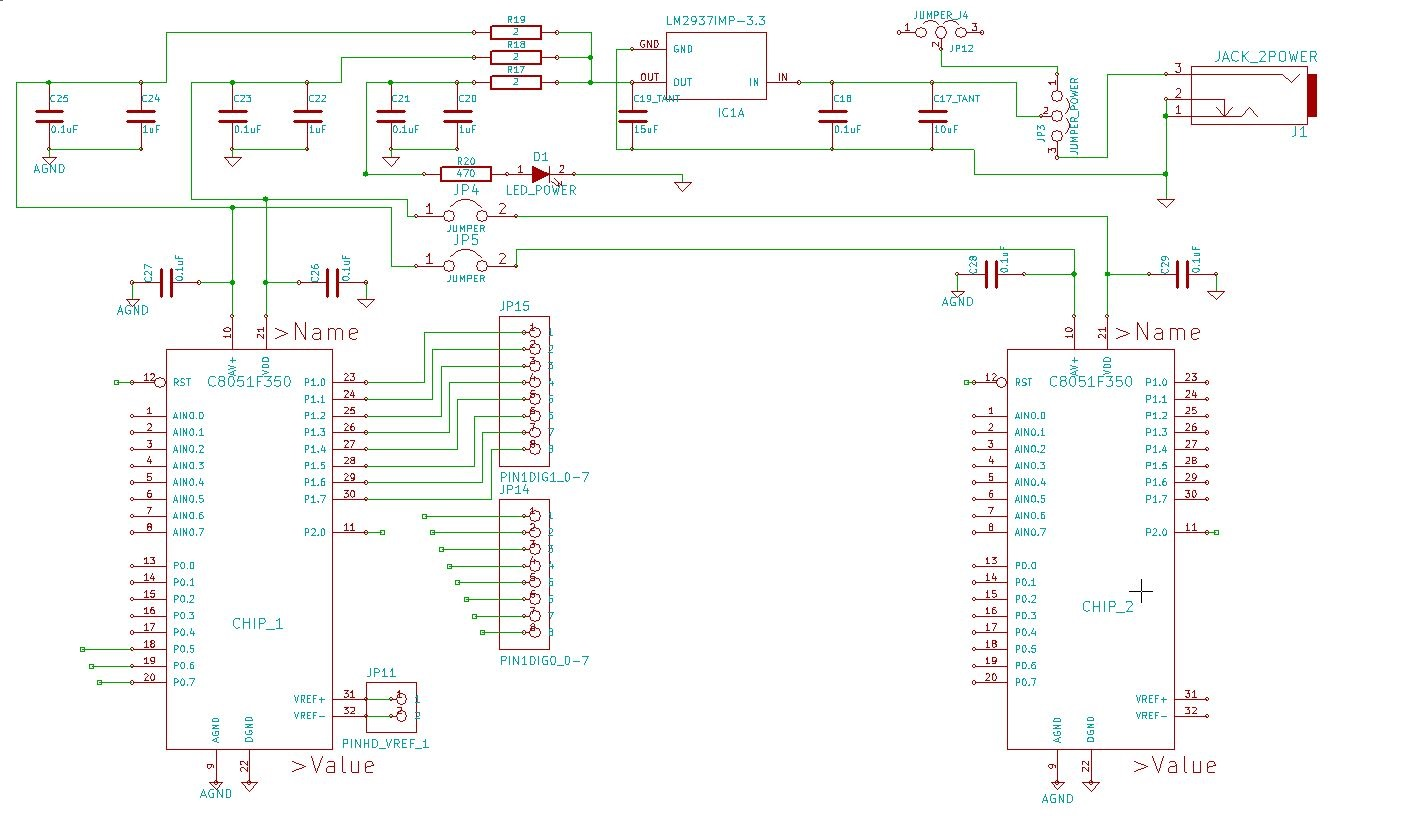
\includegraphics[width=1.0\textwidth, height = 10cm]{esquematicoPotencia2}
  \caption{Esquemático del Circuit para la potencia de alimentación.}\label{fig:esquematicoPotencia2}
\end{figure}

%subsubsection circuito_potencia2 (end)

\subsubsection{Diagrama Esquemático Completo}
\label{subsubsection: esquematico_completo2}

En la figura \ref{fig:esquematicoCompleto2} podemos ver como queda el esquemático entero con los dos microcontroladores y todos los subcircuitos que componen la placa.

\begin{figure}  
\centering
  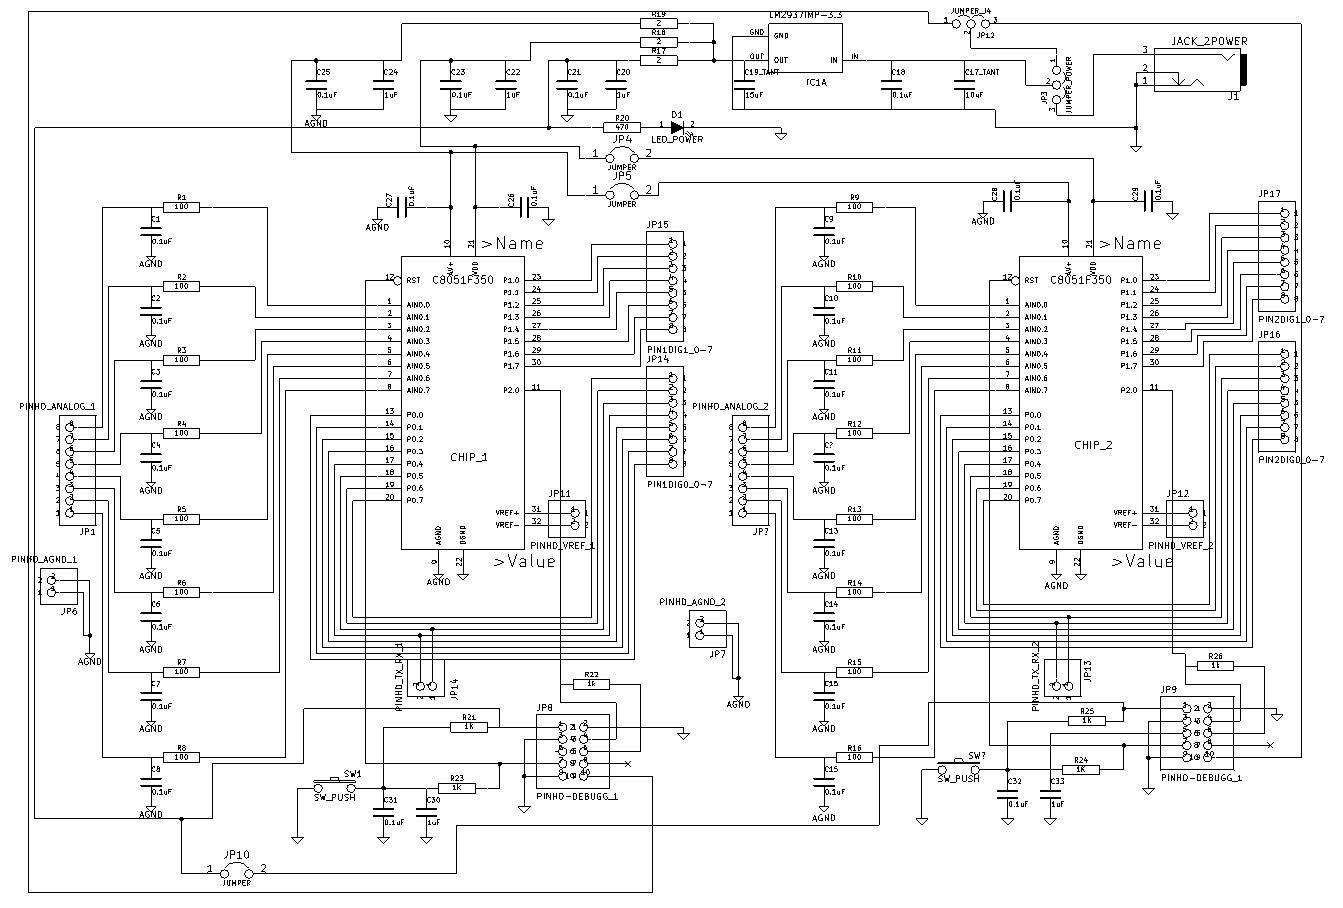
\includegraphics[width=1.10\textwidth, height = 12cm]{esquematicoCompleto2}
  \caption{Esquemático del Circuit completo de la Placa de desarrollo.}\label{fig:esquematicoCompleto2}
\end{figure}


% subsubsection esquematico_completo2 (end)

% subsection diseño_esquematico2 (end)

\subsection{Diseño de Plaqueta de Circuito Impreso (PCB)}
\label{ subsection: diseño_pcb2}

Como esta nueva versión de la placa fue diseñada para ser doble capa, se mostrarán 2 figuras, una para la capa superior y otra para la capa inferior. 
A ambas capaz le tuvimos que dividir las masas, en una sección analógica y una digital, la masa analógica de la capa superior con la de la capa inferior deben estar interconectadas, lo mismo pasa con la masa digital. Por lo que realizamos un drill (un hueco) para que las masas estén en contacto.
En la figura \ref{fig:PCB2a} podemos ver como queda el diagrama PCB de capa superior o frontal, y en la figura \ref{fig:PCB23Da} vemos la misma capa con el visualizador 3D del KiCad.

\begin{figure}[H]
\centering
  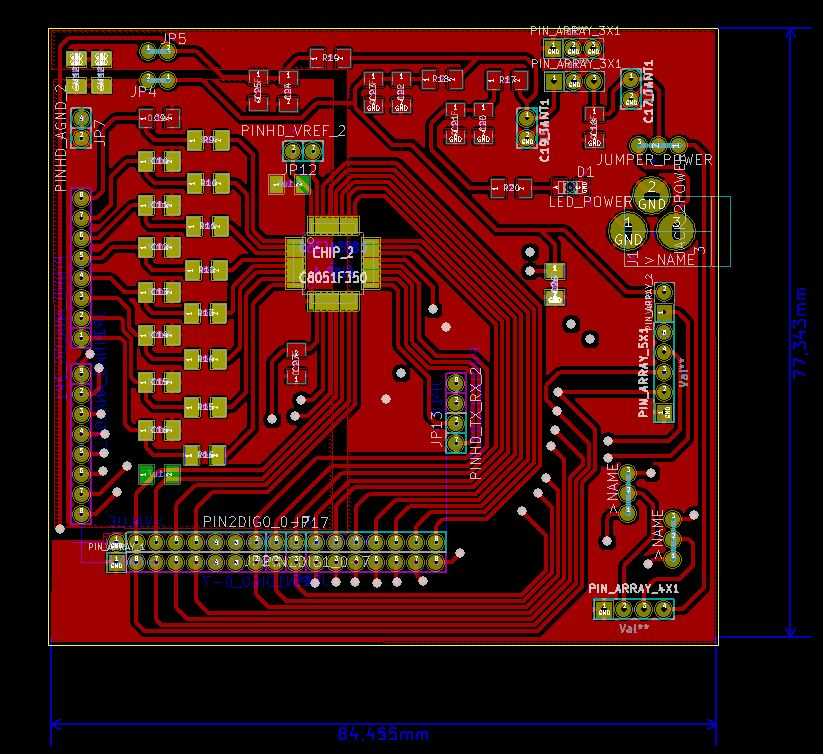
\includegraphics[width=1.0\textwidth, height = 8cm]{PCB2a}
  \caption{Diseño PCB de la capa frontal de la placa.}\label{fig:PCB2a}
\end{figure}

\begin{figure}  [H]
\centering
  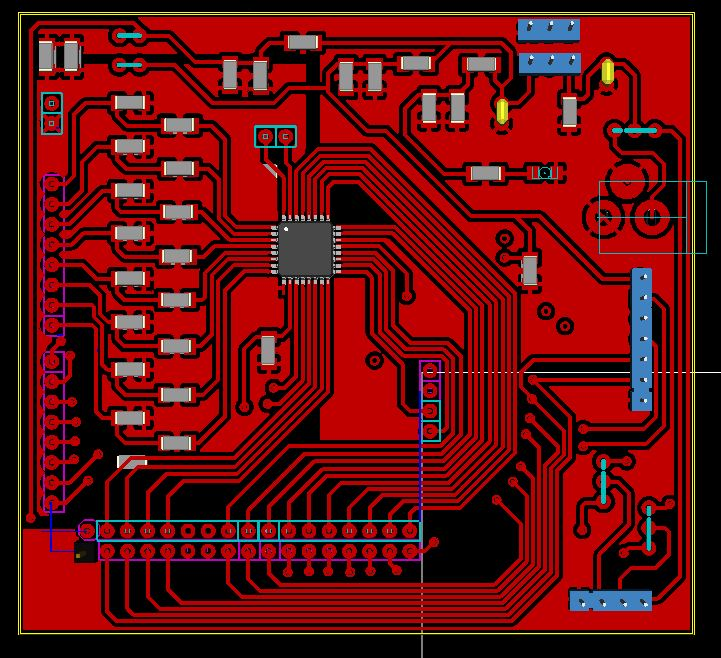
\includegraphics[width=1.0\textwidth, height = 8cm]{PCB23Da}
  \caption{Diseño PCB de la capa frontal de la placa en 3D.}\label{fig:PCB23Da}
\end{figure}

En la figura \ref{fig:PCB2b} podemos ver como queda el diagrama PCB de capa inferior o posterior, y en la figura \ref{fig:PCB23Db} vemos la misma capa con el visualizador 3D del KiCad.

\begin{figure}[H] 
\centering
  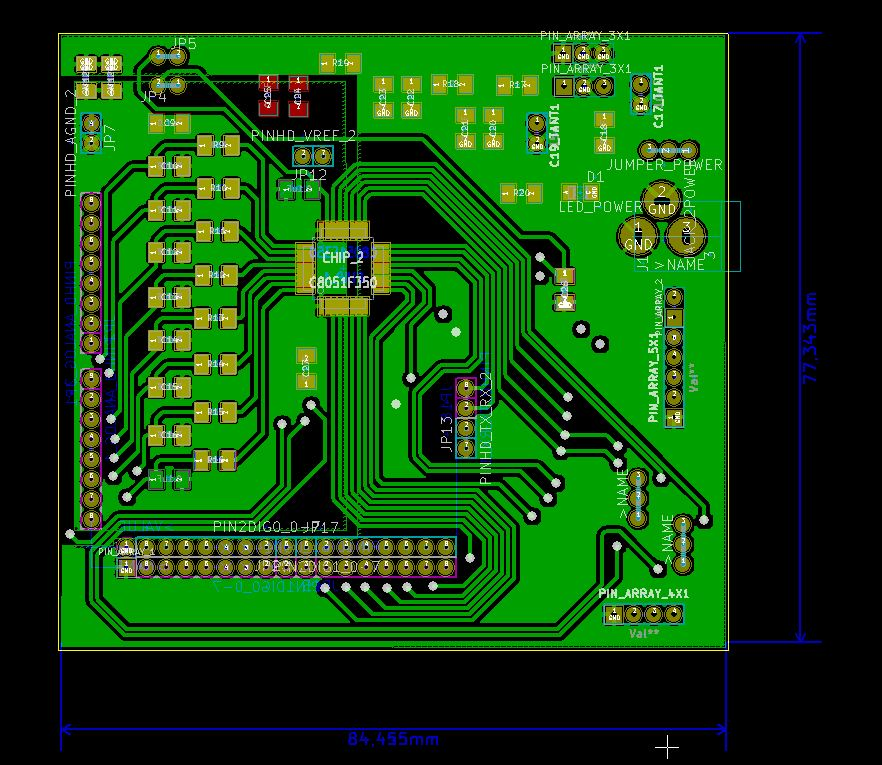
\includegraphics[width=1.0\textwidth, height = 8cm]{PCB2b}
  \caption{Diseño PCB de la capa posterior de la placa.}\label{fig:PCB2b}
\end{figure}

\begin{figure}  [H]
\centering
  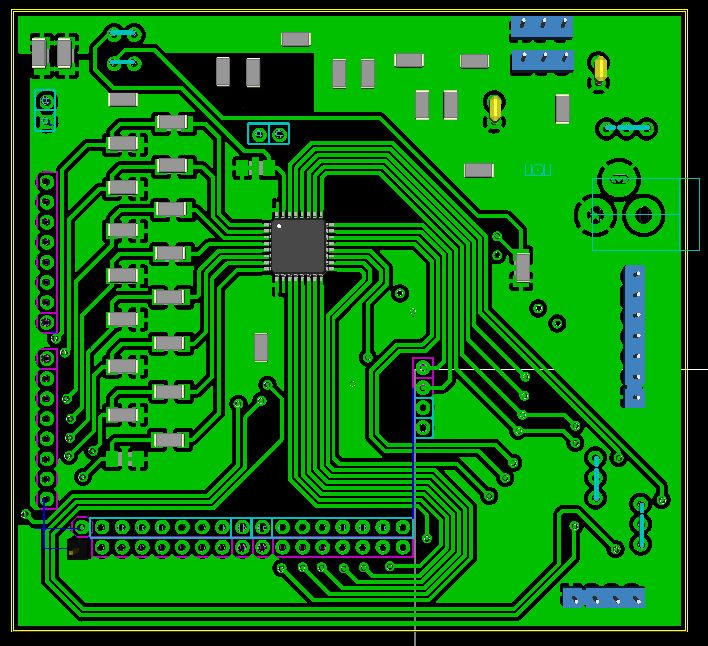
\includegraphics[width=1.0\textwidth, height = 8cm]{PCB23Db}
  \caption{Diseño PCB de la capa posterior de la placa en 3D.}\label{fig:PCB23Db}
\end{figure}


% subsection diseño_pcb2 (end)

\section{Pruebas} % (fold)
\label{sec:pruebas}

\begin{table}[h]
\caption{Test de sistema 1: Correcto Diseño de PCB.}
\label{it4:tab:testsistema1}
\begin{tabular}{p{2cm} p{9cm}}
\multicolumn{2}{c}{\cellcolor[HTML]{68CBD0}{\color[HTML]{000000} Prueba de sistema}} \\
Prueba \#        & 1 \\
\hline
Nombre           & Correcto Diseño de PCB. \\
\hline
Requerimientos  &  1.1, 1.3, 1.6, 2.2 \\
\hline
Descripción      & Se verifica la existencia de errores en el diseño utilizando el ERC (perfom design rules check) que provee el software KiCad. \\
\hline
Pre-condiciones  & \tabitem Componentes colocados y pistas ruteadas. \\
                 & \tabitem Pads numerados con sus etiquetas.  \\
\hline
Post-condiciones & El resultado de ERC deberia ser cero. \\
\hline
Resultados       & No encontramos errores de diseño en el PCB. \\                                                                           
\end{tabular}
\end{table}

\begin{table}[h]
\caption{Test de sistema 2: Correcta impresión de la placa.}
\label{it4:tab:testsistema2}
\begin{tabular}{p{2cm} p{9cm}}
\multicolumn{2}{c}{\cellcolor[HTML]{68CBD0}{\color[HTML]{000000} Prueba de sistema}} \\
Prueba \#        & 2 \\
\hline
Nombre           & Correcta impresión de la placa.   \\

\hline
Requerimientos &    1.1, 1.3, 1.6, 2.2 \\
\hline
Descripción      & Corroboramos que todas las pistas y que todos los esquemas de perforado se hayan impreso correctamente. Luego, con un multímetro en modo continuidad, comprobamos que no existan cortocircuitos entre pistas y masa o entre pads y masa. \\
\hline
Pre-condiciones  & \tabitem Placa impresa. \\
                 & \tabitem Multímetro seteado en continuidad. \\
\hline
Post-condiciones & La placa debe tener las mismas pistas que aparecen en el diseño de PCB, y al medir con el multímetro nunca debe dar continuidad entre masa y pistas, o entre pads y pistas. \\
\hline
Resultados       & Todas las pistas se correspondían con el diseño de PCB.  \\                                                                                                                               
\end{tabular}
\end{table}

\begin{table}[h]
\centering
\caption{Test de sistema 3: Correcta soldadura de Componentes.}
\label{it4:tab:testsistema3}
\begin{tabular}{p{2cm} p{9cm}}
\multicolumn{2}{c}{\cellcolor[HTML]{68CBD0}{\color[HTML]{000000} Prueba de sistema}} \\
Prueba \#        & 3 \\
\hline
Nombre           & Correcta soldadura de Componentes. \\
\hline
Requerimientos &    1.1, 1.3, 1.6, 2.2   \\
\hline
Descripción      & Se utiliza el multímetro en modo continuidad para poder comprobar si existen cortocircuitos y verificar si todos los componentes están bien interconectados. \\
\hline
Pre-condiciones  & \tabitem Placa impresa. \\
                 & \tabitem Pistas impresas correctamente. \\
                 & \tabitem Componentes soldados. \\
                 & \tabitem Multímetro seteado en continuidad. \\
\hline
Post-condiciones &  No debería haber cortocircuitos, y la interconexión entre los distintos componentes debería corresponderse con el diseño de PCB. \\ 
\hline
Resultados       & Encontramos cortocircuitos luego de soldar los componentes. Fue necesario des-soldar algunos componentes y volverlos a colocar para solucionar el problema. \\
\end{tabular}
\end{table}

\begin{table}[h]
\centering
\caption{Test de sistema 4: Correcta Comunicación Con SiliconLabs Debugger.}
\label{it4:tab:testsistema4}
\begin{tabular}{p{2cm} p{9cm}}
\multicolumn{2}{c}{\cellcolor[HTML]{68CBD0}{\color[HTML]{000000} Prueba de sistema}} \\
Prueba \#        & 4 \\
\hline
Nombre           & Correcta Comunicación Con SiliconLabs Debugger. \\
\hline
Requerimientos &  \tabitem Se debería poder conectar el debugger del microcontrolador a la placa para poder programarlo. \\
\hline
Descripción      & Se utilizo el cable USB con el debugger de SiliconLabs para conectar la placa a la PC. \\
\hline
Pre-condiciones  & 3.2 \\
\hline
Post-condiciones &  Al abrir la IDE y apretar el botón de "Connect" el programa debe reconocer el tipo de microcontrolador al que esta conectado. \\ 
\hline
Resultados       &  Conectamos la placa a la PC e intentamos conectarla con el microcontrolador a traves de la IDE. El resultado fue el esperado, el microcontrolador estaba exitosamente conectado al ordenador. \\
\end{tabular}
\end{table}

\begin{table}[h]
\centering
\caption{Test de sistema 5: Correcta programación del microcontrolador.}
\label{it4:tab:testsistema5}
\begin{tabular}{p{2cm} p{9cm}}
\multicolumn{2}{c}{\cellcolor[HTML]{68CBD0}{\color[HTML]{000000} Prueba de sistema}} \\
Prueba \#        & 4 \\
\hline
Nombre           & Correcta programación del microcontrolador. \\
\hline
Requerimientos &  3.2 \\                                   
\hline
Descripción      & Se utilizo el cable USB con el debugger de SiliconLabs para conectar la placa a la PC y descargarle un programa .hex al microcontrolador. \\
\hline
Pre-condiciones  & \tabitem Placa impresa. \\
                 & \tabitem Pistas impresas correctamente. \\
                 & \tabitem Componentes soldados. \\
                 & \tabitem IDE SiliconLabs instalada en la PC. \\
                 & \tabitem IDE SiliconLabs reconociendo el C8051f352. \\
\hline
Post-condiciones &  Al abrir la IDE y apretar el botón de "Connect" el programa debe reconocer el tipo de microcontrolador al que esta conectado y luego a través de la misma IDE o del "Flash Programing Utilitys" cargarle un programa .hex al c8051f352. \\ 
\hline
Resultados       &  Conectamos la placa a la PC y desde el software "Flash Programing Utilitys" se pudo cargar un programa a los microcontroladores soldados en la placa. \\                                                                                                  
\end{tabular}
\end{table}

\begin{table}[h]
\centering
\caption{Test de sistema 6: Correcto funcionamiento de las entradas analógicas y salidas digitales.}
\label{it4:tab:testsistema6}
\begin{tabular}{p{2cm} p{9cm}}
\multicolumn{2}{c}{\cellcolor[HTML]{68CBD0}{\color[HTML]{000000} Prueba de sistema}} \\
Prueba \#        & 4 \\
\hline
Nombre           & Correcto funcionamiento de las entradas analógicas y salidas digitales. \\                      

\hline
Requerimientos &    1.1
\hline
Descripción      & Se cargo un programa de prueba a ambos microcontroladores. Utilizando una fuente de tension, introducimos distintos valores de tension en dos canales en modo unico, uno de cada microcontrolador. Luego, utilizamos ambas plataformas para convertir los datos a digital y verificar que la telemetria medida concuerde con el nivel de tension generado.
\hline
Pre-condiciones  & \tabitem Componentes conectados y soldados correctamente en la placa. \\
                 & \tabitem IDE SiliconLabs iniciado y corriendo en un ordenador. \\
                 & \tabitem Microcontrolador conectado y reconocido por el software de Silicon Labs. \\
                 & \tabitem Programa de prueba correctamente cargado en el C8051f352. \\
                 & \tabitem Fuente de Tensión externa conectada a las entradas analógicas con referencia en masa analógica. \\
\hline
Post-condiciones &  Al apretar el botón de "Go" en el programa "Flash Programing Utilitys", se inicia el programa. Configurando los canales conectados e iniciando las conversiones continuas, deberian comenzar a aparecer las mediciones realizadas sobre los canales. Las mediciones deberian corresponderse con los valores de tension establecidos en las fuentes conectadas. \\
\hline
Resultados       &  Cargamos el programa en el microcontrolador, y con todas las pre-condiciones cumplidas hicimos correr el programa. Los valores de tension medidos se correspondian con los establecidos en la fuente. \\                                                                                                            
\end{tabular}
\end{table}


% section pruebas (end)

\section{Resultados} % (fold)
\label{sec:resultados}


Al final de esta iteracion, obtuvimos una plataforma con dos microcontroladores y el doble de recursos que la diseñada anteriormente. Esto permite con los requisitos de cantidad de contadores y cantidad de canales de conversion diferencial, ligados a los requerimientos 1.1 y 1.3.
Aun asi, todavia queda trabajo por hacer. Aunque los recursos esten duplicados, es necesario vincular ambas plataformas, para que trabajen en conjunto y no en paralelo. De esta forma, pasa a ser una unica plataforma con el doble de recursos, y no dos plataformas en un unico espacio fisico.

En esta iteracion, llegamos a unir dos plataformas en un unico lugar fisico, pero sin correlacionar su funcionamiento.

En la figura \ref{fig:impresionplaca2_a} y \ref{fig:impresionplaca2_b} podemos ver como quedo la placa final, tanto de la capa superior como de la inferior. Se acomodoaron los componentes de manera tal que los pines y módulos que se pueden utilizar para conectar alguna interfaz/cable, queden en la misma capa.

\begin{figure}  
\centering
  \includegraphics[width=1.10\textwidth, height = 12cm]{impresionplaca2_a}
  \caption{Circuito de Hardware final ya impreso.}\label{fig:impresionplaca2_a}
\end{figure}

\begin{figure}  
\centering
  \includegraphics[width=1.10\textwidth, height = 12cm]{impresionplaca2_b}
  \caption{Circuito de Hardware final ya impreso.}\label{fig:impresionplaca2_b}
\end{figure}



% section resultados (end)

% chapter iteracion_4 (end)